\section{Subsistema: Localização e Informações}
Este tópico descreve as soluções para localização do veículo no terreno da lavoura, sua trajetória e
como serão processados e armazenados os dados coletados das medições.

  \subsection{Localização}

  Pela necessidade do veículo realizar seu percurso de maneira autônoma, as soluções identificadas
  pelo grupo basearam-se em processamento de imagens, GPS e sensores de proximidade.

  Tendo em vista o curto período de tempo destinado ao desenvolvimento do projeto e a falta de
  conhecimento da equipe sobre processamento de imagens, essa opção apresentou um alto grau de risco
  e foi descartada.

  Já a opção do GPS se tornou insatisfatória para o projeto, uma vez que erros
  referentes à precisão podem acarretar em um comprometimento da plantação
  por parte do veículo.

  Dessa forma, foram feitos estudos sobre sensores de proximidade, especificamente
  ultrassom e infravermelho, os quais demonstraram ser uma solução viável e foram alvo de
  estudos mais aprofundados.

  Inicialmente, a opção baseada em ultrassom se mostrou mais adequada, porém foi possível perceber que os principais sensores
  comerciais que se baseavam nesse princípio possuíam uma faixa de detecção bastante re-
  duzida. Sendo assim, foi escolhido um sensor de proximidade baseado em infravermelho
  apresentado na figura \ref{fig:infrared}.

  \begin{figure}[!htbp]
  \begin{center}
  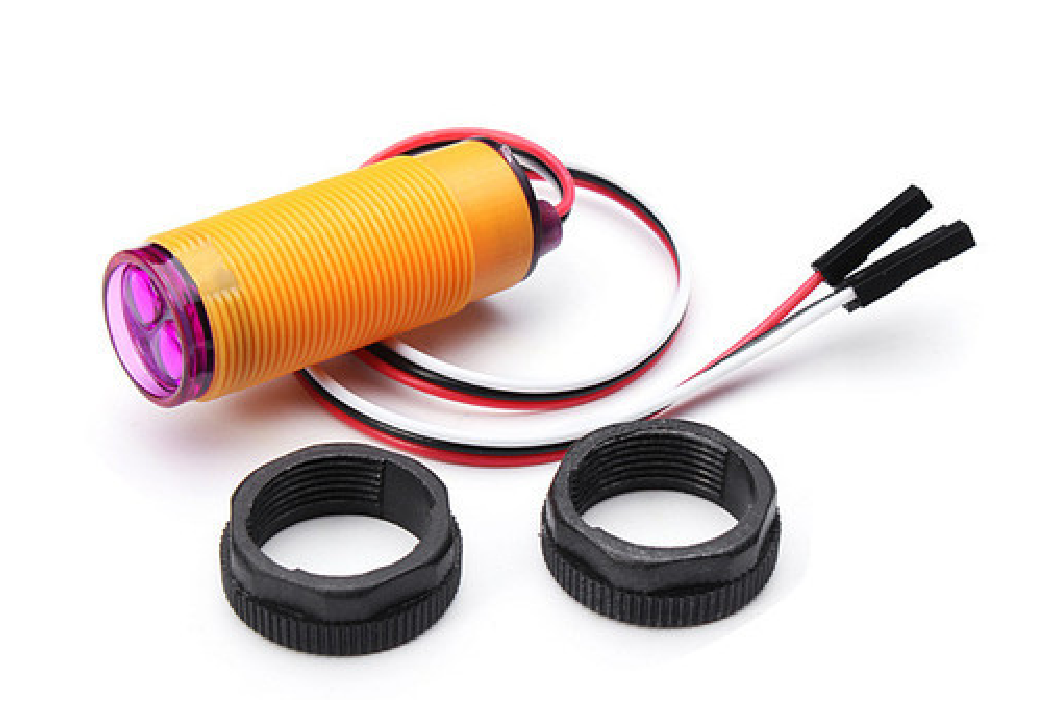
\includegraphics[width=.7\textwidth]{figuras/infrared.eps}
  \caption{\label{fig:infrared}Sensor de proximidade infravermelho.}
  \end{center}
  \end{figure}

  O princípio de funcionamento deste sensor é o princípio da triangulação.
  Um feixe de luz é emitido por um diodo laser ou um LED infravermelho.
  Ao ser refletido por um objeto, esse raio é detectado por um PSD
  (\textit{Position Sensing Device} -- Dispositivo de Monitoramento de Posição).
  De acordo com a distância do objeto que refletiu a luz, esse raio incide
  de modo diferente no PSD. A figura~\ref{fig:infrared_func} ilustra o
  princípio da triangulação.

  \begin{figure}[!htbp]
  \begin{center}
  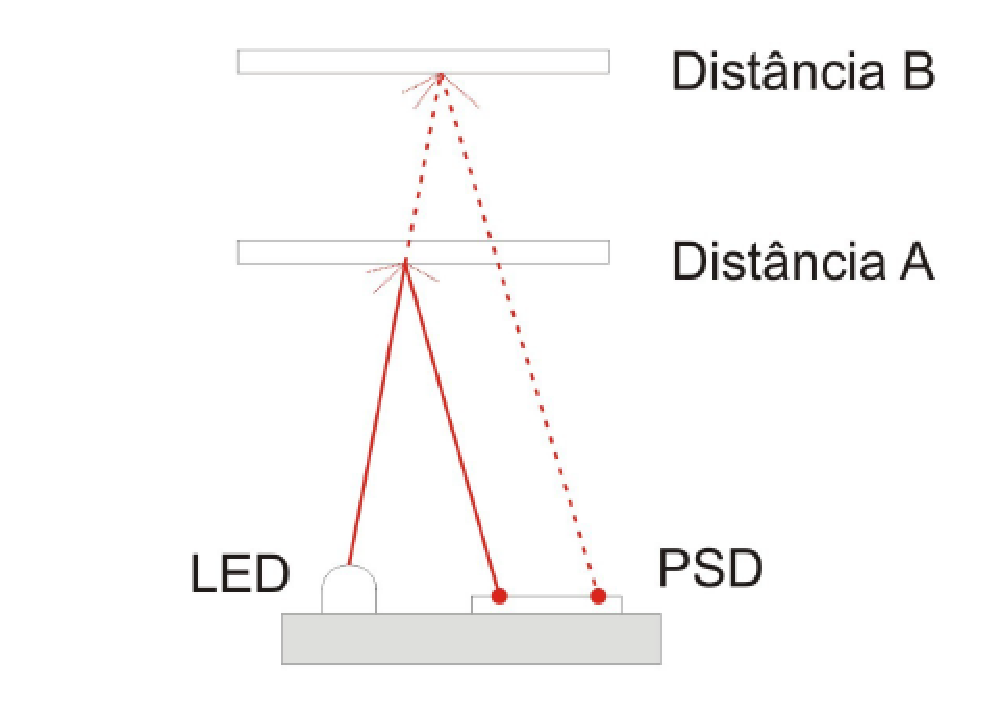
\includegraphics[width=.7\textwidth]{figuras/infrared_func.eps}
  \caption{\label{fig:infrared_func}Princípio da triangulação.}
  \end{center}
  \end{figure}

  A escolha do elemento foi motivada pela capacidade de detecção
  de proximidade ser adequada para o funcionamento do algoritmo
  de lcomoção, mais especificamente entre 3 e 80cm.  Além disso,
  este elemento apresenta pouca interferência com a luz visível e
  possui um interfaceamento simples com um microcontrolador.

  \subsection{Algoritmo de Locomoção}
    Dado a utilização de sensores infravermelho e a disposição da lavoura de morango
    é possível identificar um típico problema denominado \textit{Wall Follower}.

    Segundo \cite{huang2009}, \textit{Wall Follower},
    também conhecido como regra da mão direita ou esquerda, é válido para percursos conexos, onde todas as paredes são ligadas entre si, mantendo a mão próxima a parede do labirinto em
    que se inclui, garantindo assim que o corpo não se perca e finalize
    o percurso. O principal problema desta regra ocorre quando um percurso
    possui loops de passagens que projetem uma trajetória sem fim.

    \begin{figure}[!htbp]
    \begin{center}
    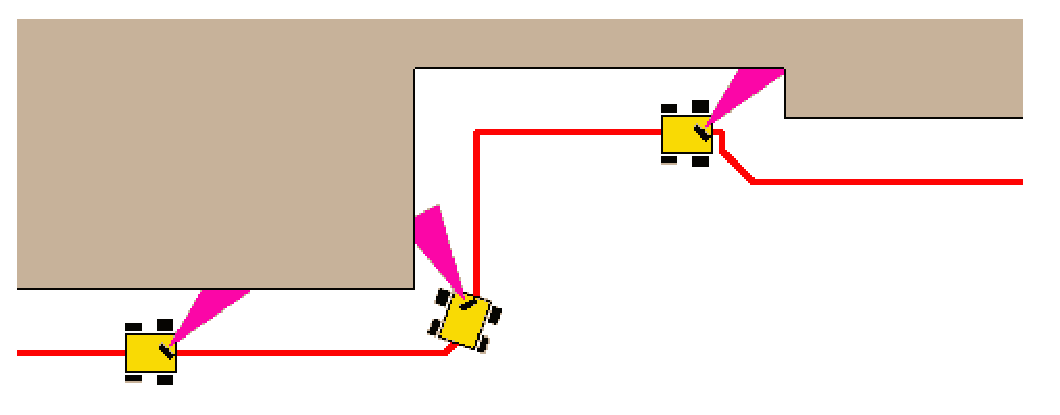
\includegraphics[width=.7\textwidth]{figuras/wallfollower.eps}
    \caption{\label{fig:wallfollower}Exemplo de \textit{Wall Follower}.}
    \end{center}
    \end{figure}

    \vfill
    \pagebreak

    Basicamente o veículo utilizará as paredes dos canteiros como guia, realizando a
    coleta de dados sempre a sua direita. Para viabilizar essa solução serão necessárias algumas adaptações no terreno com a adição de estruturas à lavoura, criando uma espécie de circuito. A figura \ref{fig:ambientadapt} representa o caminho a ser seguido pelo veículo.

    \begin{figure}[!htbp]
    \begin{center}
    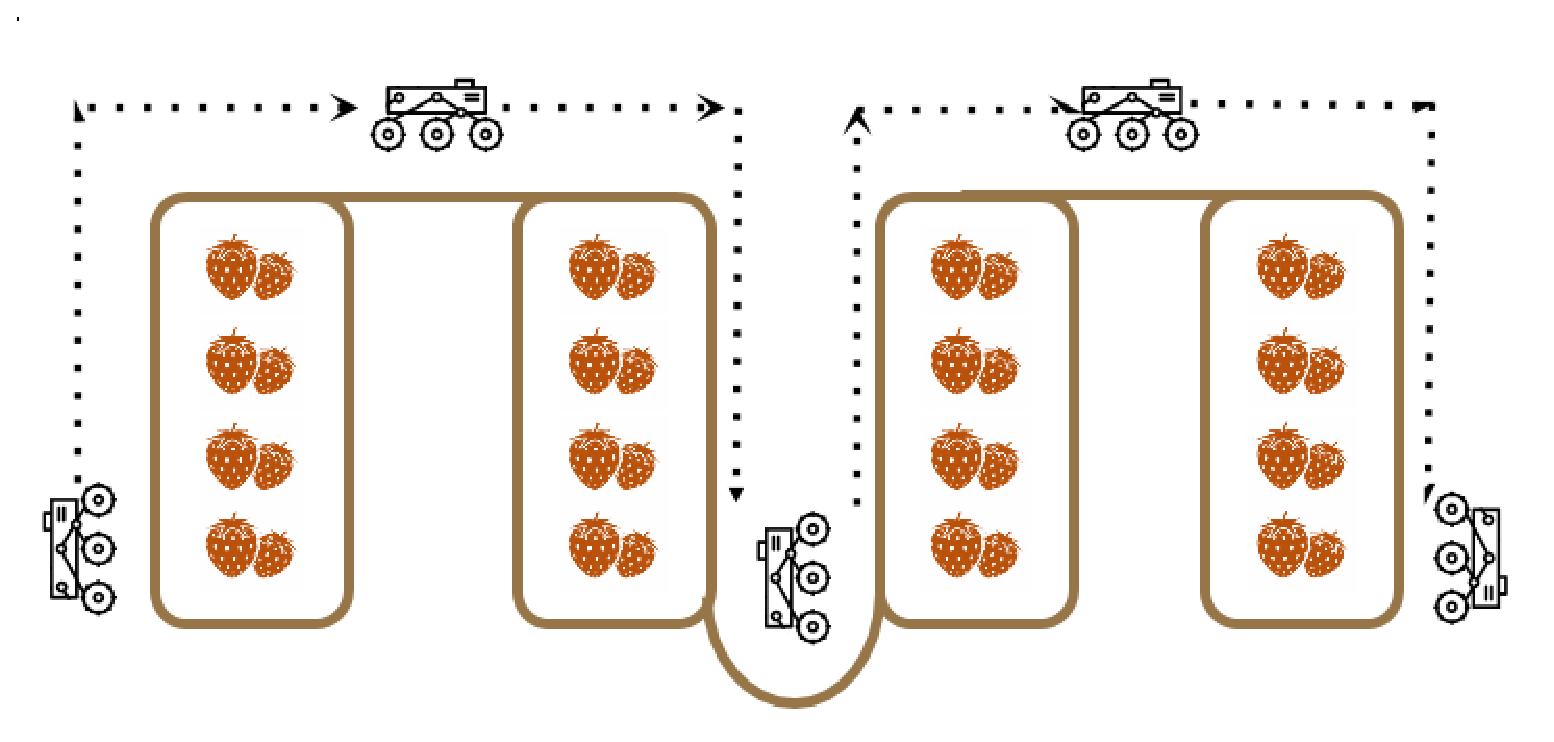
\includegraphics[width=.7\textwidth]{figuras/adapt.eps}
    \caption{\label{fig:ambientadapt}Adaptação do ambiente.}
    \end{center}
    \end{figure}

    \vfill
    \pagebreak

    Para a escolha dos componentes para a construção das barreiras ponderou-se
    necessidade de um material barato e de fácil instalação/manuseio.
    Desta forma, o plástico e a madeira foram os materiais escolhidos para compor os obstáculos
    que irão ajudar o veículo a percorrer o trajeto.

  \subsection{Informações}

  \subsubsection{Unidade de Processamento}

  Para processamento das informações foi
  escolhida foi o Raspberry Pi B+,
  É uma unidade robusta que conta com o microprocessador
  BCM2835 da Broadcom, com clock de
  700MHz e modo de baixo consumo, uma GPU Dual Core VideoCore
  IV\textregistered, SDRAM de 512MB, 4 portas USB, 1 porta RJ45
  (Ethernet), 1 porta HDMI e 40 pinos para GPIO~\cite{raspref}

  Esta unidade terá um sistema operacional Linux embarcado, responsável
  por gerenciar o armazenamento dos dados obtidos pelos sensores e
  processar decisões do controle do veículo.

  \begin{figure}[!htbp]
  \begin{center}
  \includegraphics[width=.7\textwidth]{figuras/raspberry.eps}
  \caption{\label{fig:raspberry}Raspberry Pi B+.}
  \end{center}
  \end{figure}

  \subsubsection{Armazenamento dos Dados}

  Para o armazenamento de dados foi escolhido um cartão de memória
  Micro SD de 8GB da Sandisk. Sua escolha foi motivada devido à
  necessidade de um dispositivo de armazenamento portátil, capaz de
  armazenar os dados adquiridos a partir dos sensores para a posterior
  análise. Além disso, a placa microprocessadora escolhida oferece
  suporte para cartão de memória, dispensando o uso de um módulo avulso
  para a realização das operações de armazenamento. A figura~\ref{fig:sdcard}
  apresenta o cartão de memória.

  \begin{figure}[!htbp]
  \begin{center}
  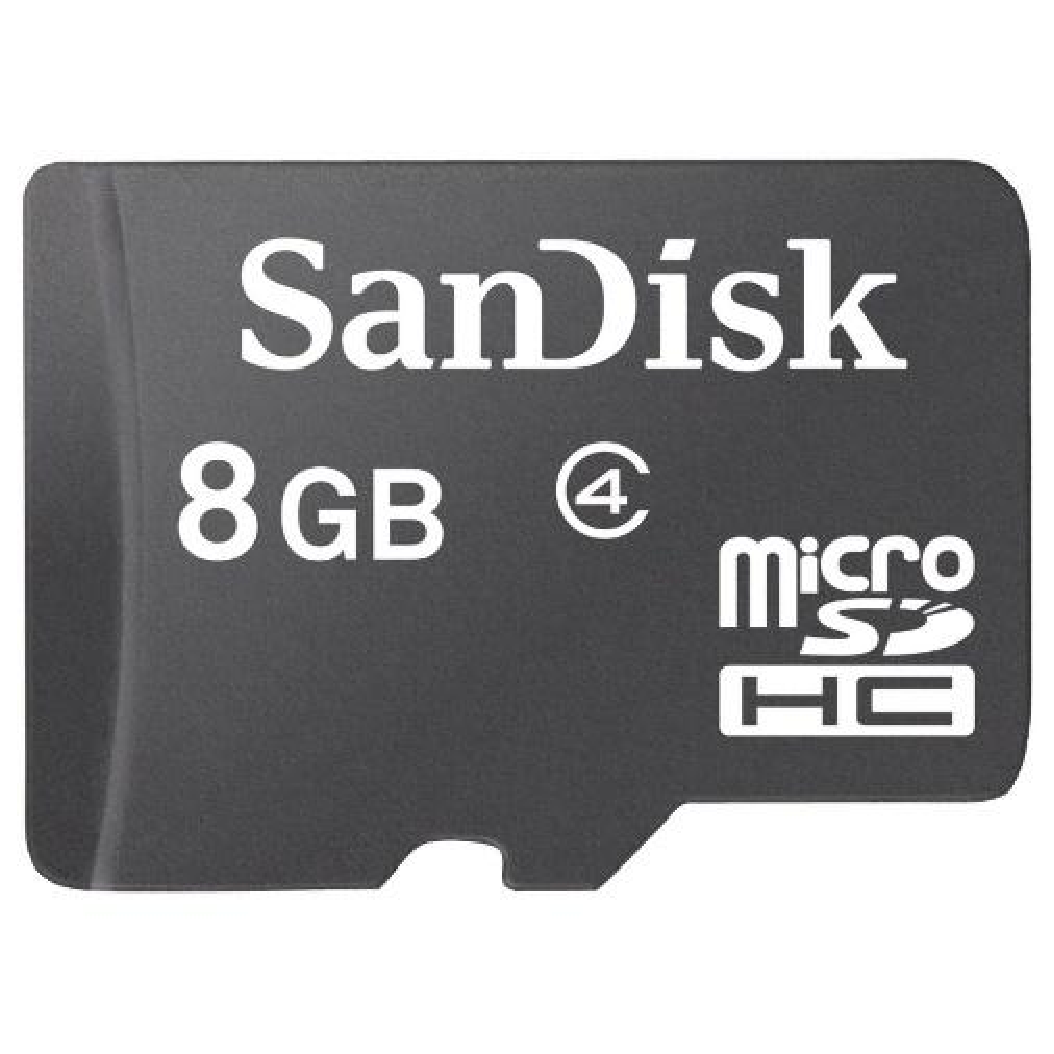
\includegraphics[width=.5\textwidth]{figuras/sdcard.eps}
  \caption{\label{fig:sdcard}Cartão de memória.}
  \end{center}
  \end{figure}

  Os dados serão armazenados no cartão de memória da Raspberry Pi
  em um arquivo no formato CSV (\textit{Comma Separated Value}). Os dados
  serão dispostos em colunas com a seguinte ordem: posição da medição
  em metros, umidade do solo, umidade relativa do ar e temperatura do
  ambiente.
  Os dados dispostos desta maneira facilitam o processamento e
  análise posterior, assim como sua apresentação gráfica para
  o operador.

  \subsubsection{Apresentação das Informações}

  Uma parte importante do projeto consiste na apresentação dos
  dados para o usuário encarregado pela gestão da lavoura. Para essa demanda,
  foi definido o desenvolvimento de uma aplicação web, utilizando
  o \textit{framework} Rails.

  A escolha de desenvolver utilizando-se essa linguagem junto a
  esse \textit{framework} foi feita com base na facilidade que essa
  tecnologia fornece para o desenvolvimento e com base na experiência
  da equipe responsável pelo desenvolvimento da aplicação, visto que
  todos os membros do grupo já possuem experiência com a tecnologia.

  Em concordância com os requisitos estabelecidos, essa aplicação
  permitirá o upload do arquivo CSV gerado pelo veículo, dentro de
  uma área restrita da aplicação, disponível apenas após a realização
  do login.
  Após a realização do upload, o usuário possuirá a opção de visualizar
  os dados de forma gráfica, sendo que a visualização gráfica se dará
  com base em um heatmap (mapa de calor) para uma melhor representação
  da lavoura.
  Além da representação gráfica, o gestor da lavoura poderá obter
  esses dados em formato de relatório, sendo permitida sua
  exportação para um arquivo PDF (Portable Document Format).
